\begin{frame}{Fonds Charcot\footnote{\url{https://patrimoine.sorbonne-universite.fr/collection}}}
	
{
	\setbeamercolor{block body}{bg=white}
	\setbeamercolor{block title}{bg=blue}
	
	\begin{block}{SorbonNum\\
			\footnotesize{Bibliothèque de Sorbonne Université (\textsc{BSU})}}
		201 documents XML OCRisés (sans post-correction)
	\end{block}
}
%\begin{itemize}
%    \item \textrm{Charcot} : textes rédigés par Charcot
%    \item \textrm{Autres} : textes rédigés par les membres de son réseau scientifique
%\end{itemize}
\begin{table}[!ht]
	\centering
		
		\resizebox{\textwidth}{!}{  
	\begin{tabular}{|c|r|r|r|r|r|r|r|}
		\hline 
	
		\rowcolor{yellow!30}
		Corpus & \multicolumn{1}{c|}{Docs} & \multicolumn{1}{c|}{Tokens\footnote{\url{https://spacy.io/models/fr\#fr_core_news_lg}}} & \multicolumn{1}{c|}{\%} & \multicolumn{1}{c|}{Types} & \multicolumn{1}{c|}{Lemmes} & \multicolumn{1}{c|}{Diversité} & \multicolumn{1}{c|}{Mémoire (Mo)} \\
		\hline
%		\begin{tabular}[c]{@{}c@{}}\textrm{Charcot}\\ \scriptsize{textes rédigés par Charcot}\end{tabular}
		
		 Charcot\textcolor{blue}{*} & 68 & 15 025 612 & 38,27 & 1 147 371 & 809 611 & 7,64 & 130,9\\
		\hline
%		\multicolumn{8}{|l|}{\small \textcolor{blue}{*} textes rédigés par Charcot} \\
%		\begin{tabular}[c]{@{}c@{}}\textrm{Autres}\\ \scriptsize{textes rédigés par les membres} \vspace{-0.15cm} \\ \scriptsize{de son réseau scientifique}\end{tabular}  
\hline
		Autres\textcolor{blue}{**}   & 133 & 24 232 207 & 61,73 & 1 773 538 & 1 218 074 & 7,32 & 179,6 \\ \hline
%		\multicolumn{8}{|l|}{\small \textcolor{blue}{**} textes rédigés par les membres de son réseau scientifique} \\
		\hline
		\textbf{Total} & \textbf{201} & \textbf{39 257 819} & \textbf{100} & \textbf{2 920 909} & \textbf{2 027 685} & \textbf{14,96} & \textbf{310,5} \\
%		\textbf{Total} & \textbf{201} & \textbf{31 979 479} (100\%)\\
		\hline
	\end{tabular}
}
	\caption{Description du corpus d'étude.
		%    \footnote{\tiny{\url{https://patrimoine.sorbonne-universite.fr/collection/Fonds-Charcot}}}
	}
	\label{tab:my_label}
\end{table}

{\small \textcolor{blue}{*} textes rédigés par Charcot \\
	{\small \textcolor{blue}{**} textes rédigés par son réseau scientifique}}
\end{frame}

\begin{frame}{Distribution des ouvrages du fonds Charcot}
	Entre 1825 et 1934. 
	\begin{itemize}
		\item corpus \textrm{Charcot} : fin \textsc{XIX}\ieme{}-début \textsc{XX}\ieme{} s. (1881-1907)
		\item corpus \textrm{Autres} : période plus longue (1825-1934)
	\end{itemize}
	
		\begin{figure}[h]
		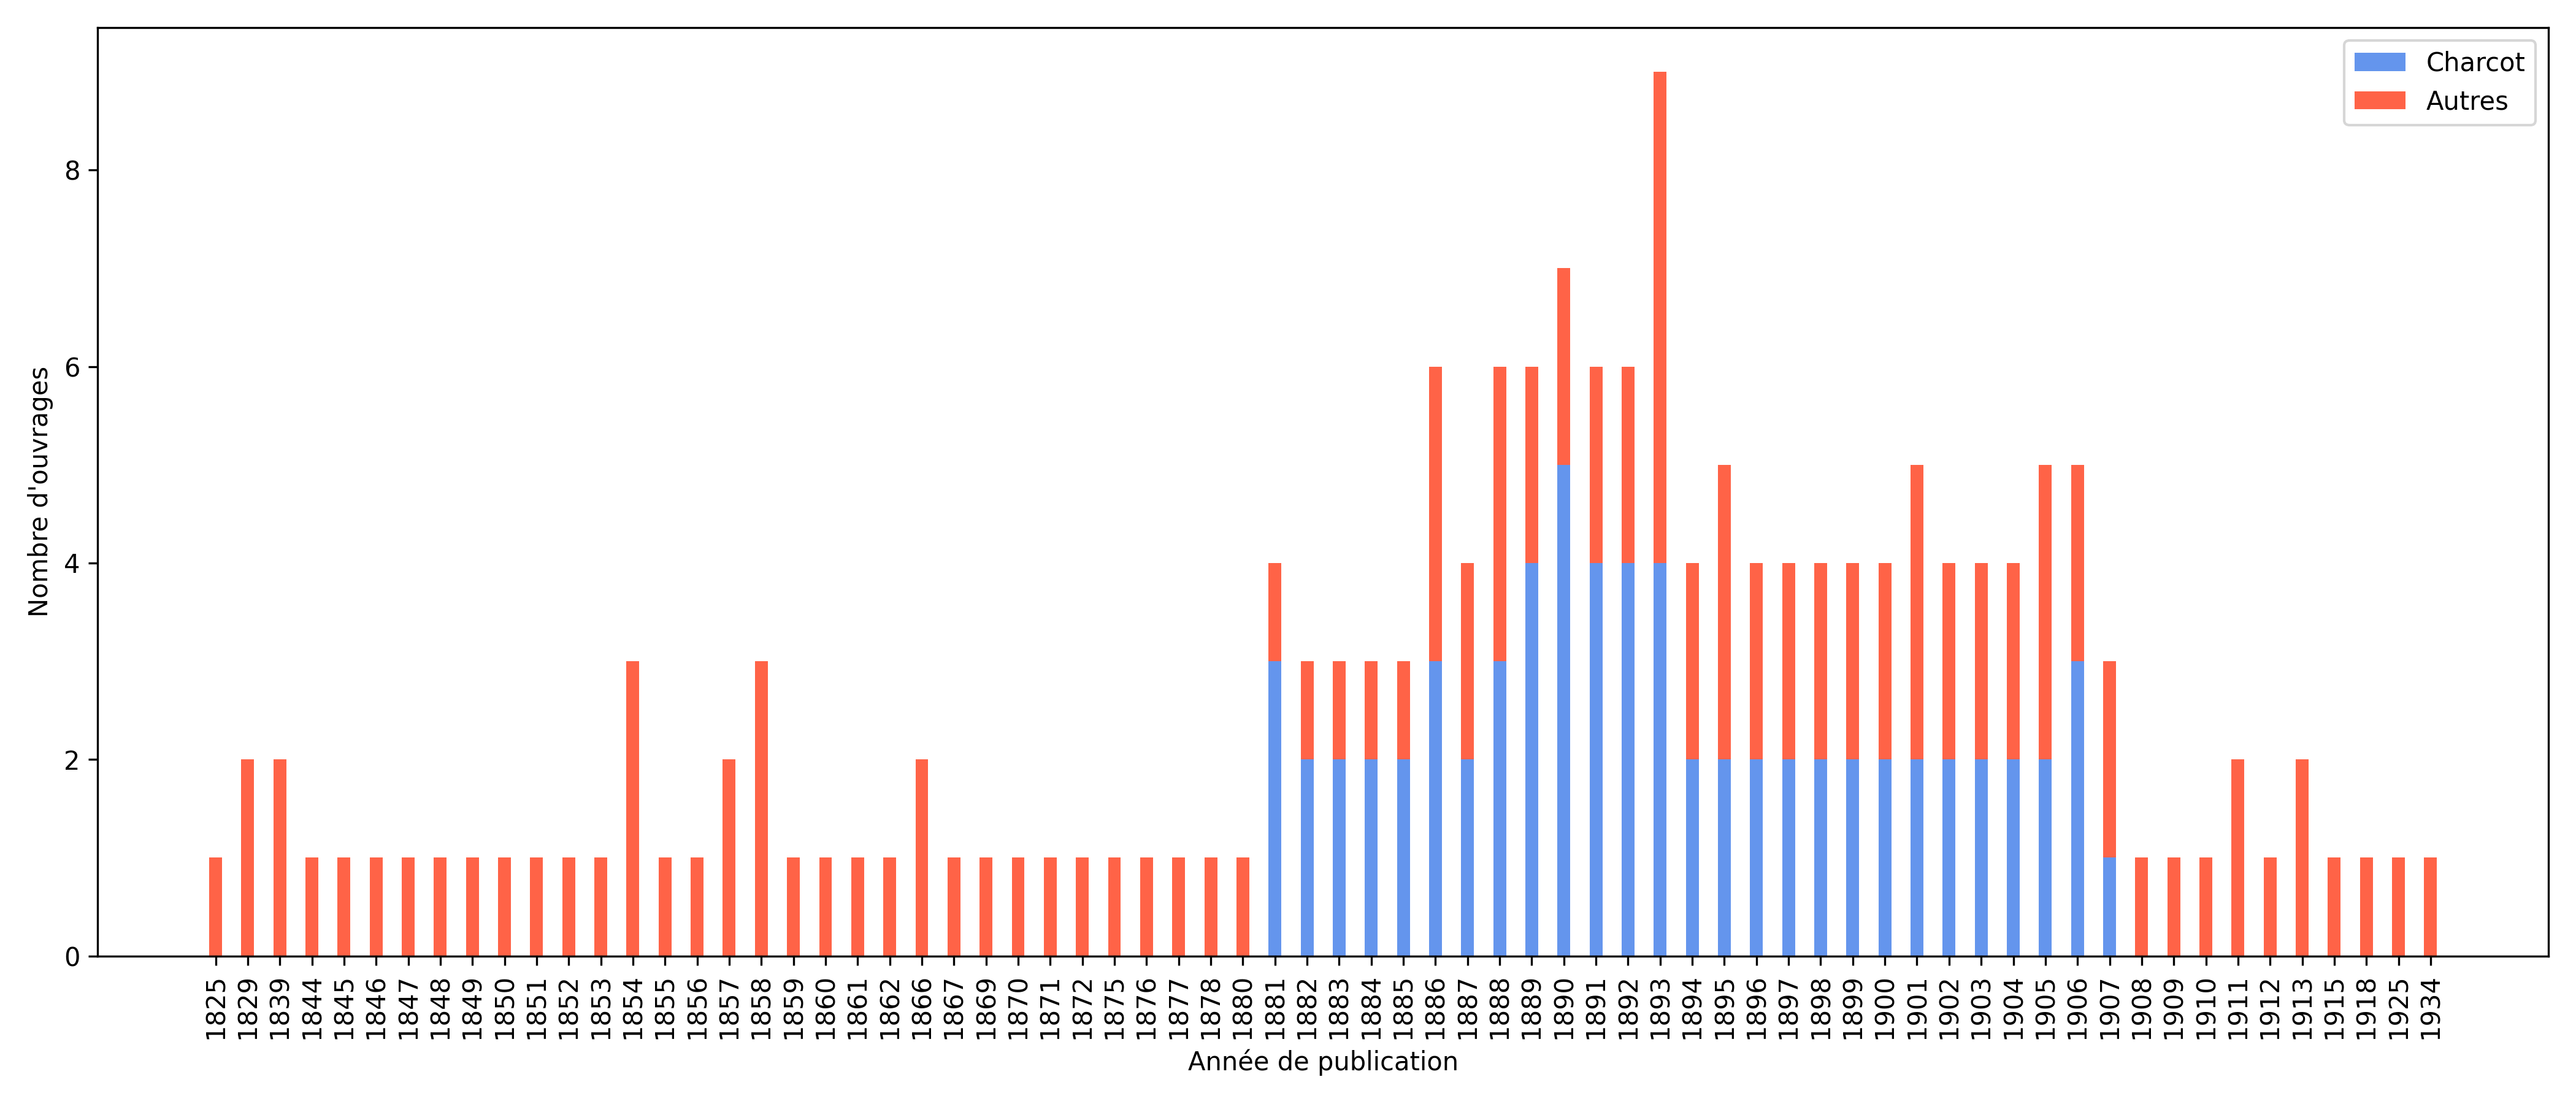
\includegraphics[width=\linewidth]{pic/distribution_ouvrages.png}
		\caption{Répartition des ouvrages constituant les corpus \og{}Charcot\fg{} et \og{}Autres\fg{} par année.}
		\label{fig:ling_out_TAL}
	\end{figure}
\end{frame}